\sectionbreak \section{ \standartTitleFont
  Введение
}

\subsection{ \standartTitleFont
  Назначения проекта
}

{\standartFont

  \par Проект предназначен для прогнозирования данных временных рядов технологического процесса пастеризационной установки в режиме реального времени и развёртывания его на программируемом микроконтроллере архитектуры PLCnext. Данный проект является модулем прогнозирования данных временных рядов технологического процесса пастеризационной уставноки. 

  \par 
}

\subsection{ \standartTitleFont
  Требования к модулю прогнозирования и постановка задачи 
}

{\standartFont

  \par Модуль прогнозирования должен выполнять прогноз технологического процесса пастеризационной установки. Для этого ему необходимо получать данные технологического процесса пастеризационной установки с помощью программируемого микроконтроллера, использующего платформу PLCnext Technology. По этой причине, программа должна быть написана на низкоуровневом языке программирования, а именно на C++, который поддерживается данным микроконтроллером.

  \par Поскольку процесс пастеризации происходит непрерывно, то программа должна работать в режиме реального времени и своевременно снабжать необходимой информацией о прогнозах поведения пастеризационной установки.

  \par Программа должно быть устойчива к различным сбоям и авариям, а также не создавать их сама.

  \par Для постановки задачи, необходимо понимать, что сама программа, которая будет в дальнейшем использоваться для прогнозирования данных временных рядов технологического процесса пастеризационной установки, будет использовать нейросетевое решение задачи прогнозирования. Для обучения модели нейронной сети применяются алгоритмы машинного обучения, от которых зависит качество модели прогнозирования. Оттого данная работа в основном и будет развиваться по этапам инженерии машинного обучения, и потому данная работа будет являться проектом машинного обучения.

  \par Задачей для проекта машинного обучения будет является разработка модуля прогнозирования данных временных рядов пастеризационной установки с целью прогноза поведения пастеризационной установки, планирования производства, а также выявления аномального поведения, возможных сбоев и выбросов пастеризационной установки.

  \par Для выполнения поставленной задачи необходимо изучать данные технологического процесса, а также провести их анализ и обработку. Далее необходимо выбрать подходящую архитектуру нейронной сети, построить и обучить модель сети, после чего организовать эффективное обучение сети, используя алгоритмы машинного обучения. Написать код нейронной сети необходимо на низкоуровневом языке программирования для дальнейшего развёртывания на программируемом контроллере, взаимодействующим с пастеризационной установкой.

  \par Также необходимо произвести тестирование и оценку качества полученной модели. После чего непосредственно выполнить процесс развёртывания нейронной сети.

  \par
}

\subsection{ \standartTitleFont
  Технические особенности проекта
}

{\standartFont

  \par Проект написан в основном на низкоуровневом языке программирования С++20 с использованием кроссплатформенной утилиты Cmake. 

  \par Проект использует также и высокоуровневый язык программирования Python для визуализации данных. В случае, если поддержки Python не будет, то не будет возможности визуализировать данные. 

  \par Документация к проекту создана с помощью XeLaTeX. 

  \par 
}

\subsection{ \standartTitleFont
  Структура проекта 
}

{\standartFont

  \par  

  \par 
}


\subsection{ \standartTitleFont
  Анализ имеющихся данных 
}


{\standartFont

  \par Модуль DataManipulator предназначен для различного рода обработки данных, с целью получения наборов данных (датасетов) необходимых для обучения моделей неройнных сетей. DataManipulator помогает преодолеть этап анализа и обработки данных, а также этап конструирования признаков.

  \par

  \begin{sidewaysfigure}
    \centering
    \def\svgwidth{\textwidth}
    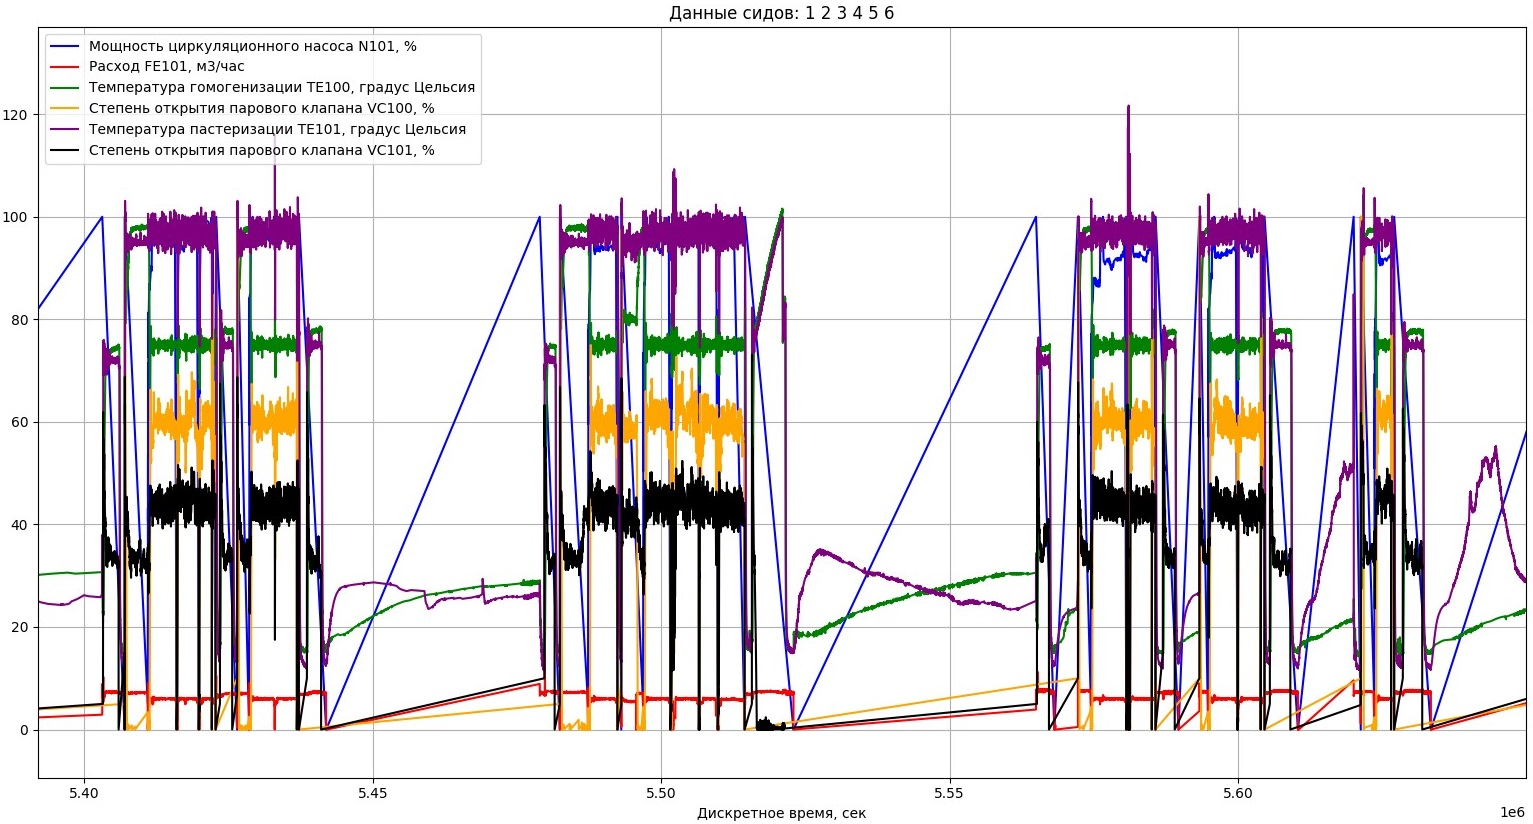
\includegraphics[scale=0.6]{images/forGeneral/data_1_visual.jpg}
    \caption{Визуализация данных 1-ого файла}
    \label{fig:Data1Visual}
  \end{sidewaysfigure} 

  \begin{sidewaysfigure}
    \centering
    \def\svgwidth{\textwidth}
    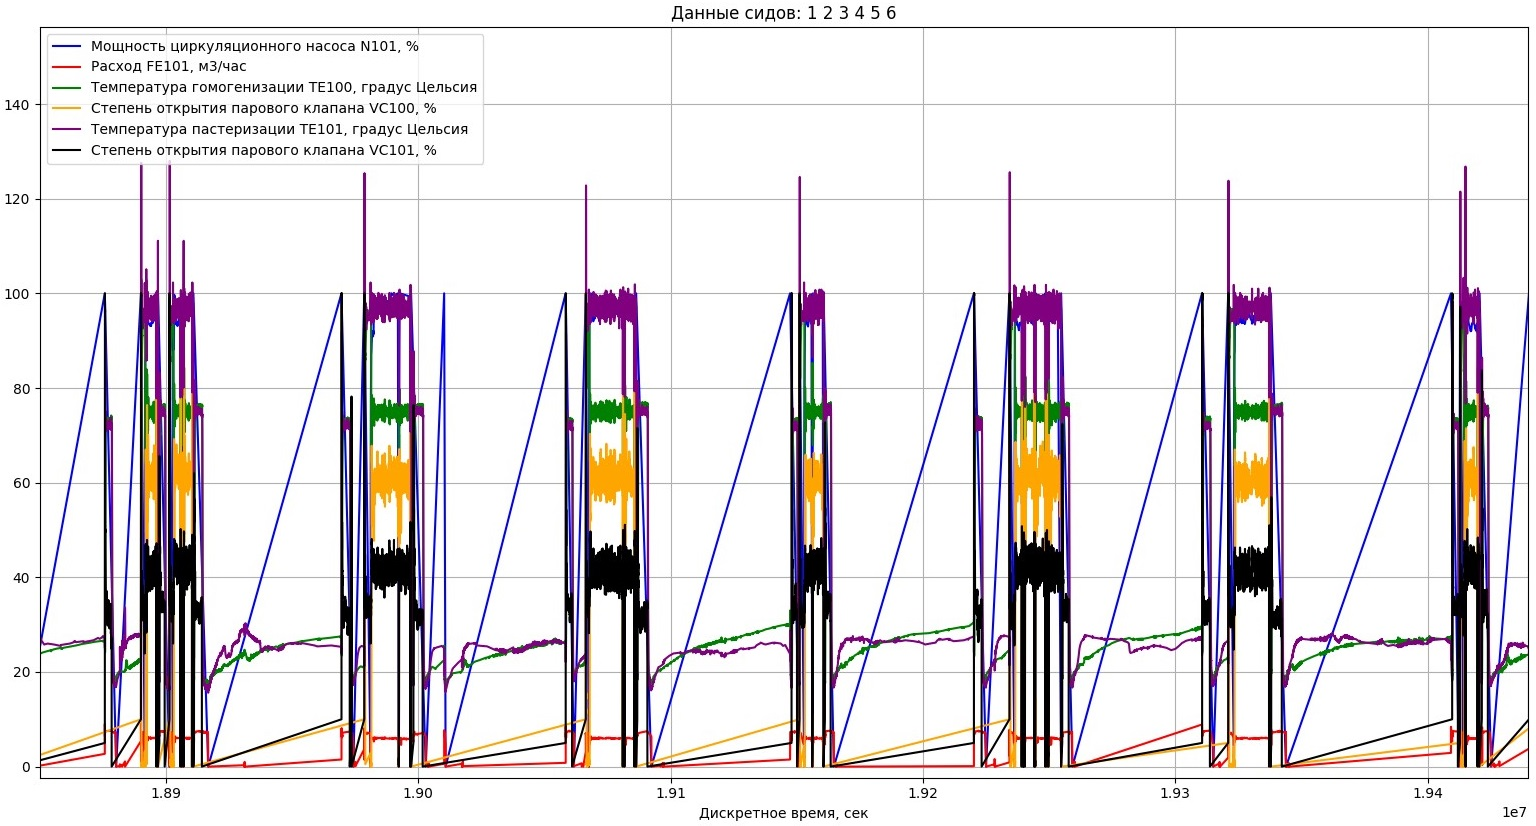
\includegraphics[scale=0.6]{images/forGeneral/data_2_visual.jpg}
    \caption{ Визуализация данных 2-ого файла с растянутым масштабом по оси абсцисс}
    \label{fig:Data2Visual}
  \end{sidewaysfigure} 

  \begin{sidewaysfigure}
    \centering
    \def\svgwidth{\textwidth}
    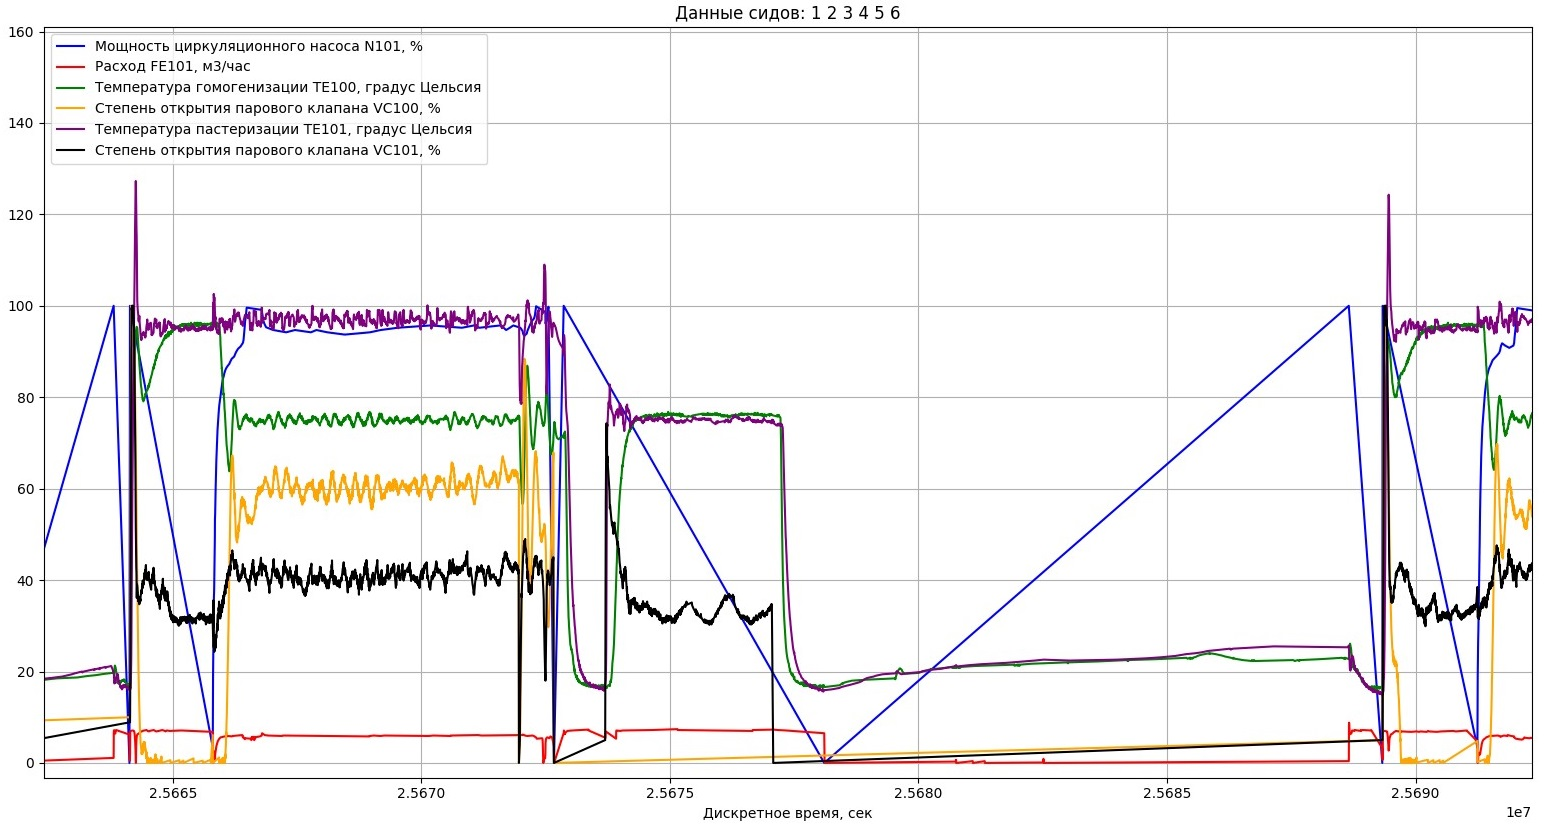
\includegraphics[scale=0.6]{images/forGeneral/data_3_visual.jpg}
    \caption{ Визуализация данных 3-ого файла с cуженным масштабом по оси абсцисс}
    \label{fig:Data3Visual}
  \end{sidewaysfigure} 

}